\documentclass[border=5pt]{standalone}
    \usepackage{tikz}
    \usetikzlibrary{arrows.meta}
    \begin{document}
    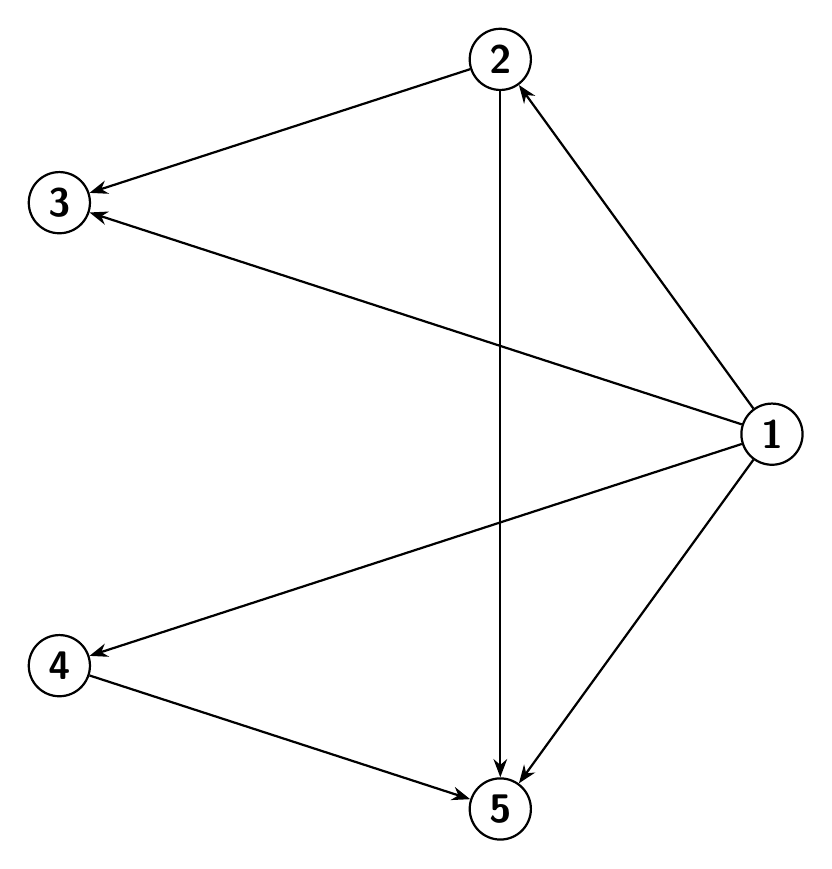
\begin{tikzpicture}[->, >=Stealth, auto, node distance=2.5cm, thick,
        main node/.style={circle, draw, font=\sffamily\Large\bfseries}]

        % Wierzcho�ki
    \node[main node] (1) at (5.00,0.00) {1};
    \node[main node] (2) at (1.55,4.76) {2};
    \node[main node] (3) at (-4.05,2.94) {3};
    \node[main node] (4) at (-4.05,-2.94) {4};
    \node[main node] (5) at (1.55,-4.76) {5};

    % Kraw�dzie
    \path (1) edge[] (2);
    \path (1) edge[] (3);
    \path (1) edge[] (5);
    \path (2) edge[] (5);
    \path (1) edge[] (4);
    \path (2) edge[] (3);
    \path (4) edge[] (5);
\end{tikzpicture}
    \end{document}